\documentclass[a4paper,12pt,twoside]{memoir}

% Castellano
\usepackage[spanish,es-tabla]{babel}
\selectlanguage{spanish}
\usepackage[utf8]{inputenc}
\usepackage[T1]{fontenc}
\usepackage{lmodern} % Scalable font
\usepackage{microtype}
\usepackage{placeins}

\usepackage {dirtytalk}
\usepackage{siunitx}

\RequirePackage{booktabs}
\RequirePackage[table]{xcolor}
\RequirePackage{xtab}
\RequirePackage{multirow}

% Links
\PassOptionsToPackage{hyphens}{url}\usepackage[colorlinks]{hyperref}
\hypersetup{
	allcolors = {red}
}

% Ecuaciones
\usepackage{amsmath}

% Rutas de fichero / paquete
\newcommand{\ruta}[1]{{\sffamily #1}}

% Párrafos
\nonzeroparskip

% Huérfanas y viudas
\widowpenalty=5000
\clubpenalty=10000

% Imagenes
\usepackage{graphicx}
\newcommand{\imagen}[2]{
	\begin{figure}[!h]
		\centering
		\includegraphics[width=0.9\textwidth]{#1}
		\caption{#2}\label{fig:#1}
	\end{figure}
	\FloatBarrier
}

\newcommand{\imagenflotante}[2]{
	\begin{figure}%[!h]
		\centering
		\includegraphics[width=0.9\textwidth]{#1}
		\caption{#2}\label{fig:#1}
	\end{figure}
}



% El comando \figura nos permite insertar figuras comodamente, y utilizando
% siempre el mismo formato. Los parametros son:
% 1 -> Porcentaje del ancho de página que ocupará la figura (de 0 a 1)
% 2 --> Fichero de la imagen
% 3 --> Texto a pie de imagen
% 4 --> Etiqueta (label) para referencias
% 5 --> Opciones que queramos pasarle al \includegraphics
% 6 --> Opciones de posicionamiento a pasarle a \begin{figure}
\newcommand{\figuraConPosicion}[6]{%
  \setlength{\anchoFloat}{#1\textwidth}%
  \addtolength{\anchoFloat}{-4\fboxsep}%
  \setlength{\anchoFigura}{\anchoFloat}%
  \begin{figure}[#6]
    \begin{center}%
      \Ovalbox{%
        \begin{minipage}{\anchoFloat}%
          \begin{center}%
            \includegraphics[width=\anchoFigura,#5]{#2}%
            \caption{#3}%
            \label{#4}%
          \end{center}%
        \end{minipage}
      }%
    \end{center}%
  \end{figure}%
}

%
% Comando para incluir imágenes en formato apaisado (sin marco).
\newcommand{\figuraApaisadaSinMarco}[5]{%
  \begin{figure}%
    \begin{center}%
    \includegraphics[angle=90,height=#1\textheight,#5]{#2}%
    \caption{#3}%
    \label{#4}%
    \end{center}%
  \end{figure}%
}
% Para las tablas
\newcommand{\otoprule}{\midrule [\heavyrulewidth]}
%
% Nuevo comando para tablas pequeñas (menos de una página).
\newcommand{\tablaSmall}[5]{%
 \begin{table}
  \begin{center}
   \rowcolors {2}{gray!35}{}
   \begin{tabular}{#2}
    \toprule
    #4
    \otoprule
    #5
    \bottomrule
   \end{tabular}
   \caption{#1}
   \label{tabla:#3}
  \end{center}
 \end{table}
}

%
% Nuevo comando para tablas pequeñas (menos de una página).
\newcommand{\tablaSmallSinColores}[5]{%
 \begin{table}[H]
  \begin{center}
   \begin{tabular}{#2}
    \toprule
    #4
    \otoprule
    #5
    \bottomrule
   \end{tabular}
   \caption{#1}
   \label{tabla:#3}
  \end{center}
 \end{table}
}

\newcommand{\tablaApaisadaSmall}[5]{%
\begin{landscape}
  \begin{table}
   \begin{center}
    \rowcolors {2}{gray!35}{}
    \begin{tabular}{#2}
     \toprule
     #4
     \otoprule
     #5
     \bottomrule
    \end{tabular}
    \caption{#1}
    \label{tabla:#3}
   \end{center}
  \end{table}
\end{landscape}
}

%
% Nuevo comando para tablas grandes con cabecera y filas alternas coloreadas en gris.
\newcommand{\tabla}[6]{%
  \begin{center}
    \tablefirsthead{
      \toprule
      #5
      \otoprule
    }
    \tablehead{
      \multicolumn{#3}{l}{\small\sl continúa desde la página anterior}\\
      \toprule
      #5
      \otoprule
    }
    \tabletail{
      \hline
      \multicolumn{#3}{r}{\small\sl continúa en la página siguiente}\\
    }
    \tablelasttail{
      \hline
    }
    \bottomcaption{#1}
    \rowcolors {2}{gray!35}{}
    \begin{xtabular}{#2}
      #6
      \bottomrule
    \end{xtabular}
    \label{tabla:#4}
  \end{center}
}

%
% Nuevo comando para tablas grandes con cabecera.
\newcommand{\tablaSinColores}[6]{%
  \begin{center}
    \tablefirsthead{
      \toprule
      #5
      \otoprule
    }
    \tablehead{
      \multicolumn{#3}{l}{\small\sl continúa desde la página anterior}\\
      \toprule
      #5
      \otoprule
    }
    \tabletail{
      \hline
      \multicolumn{#3}{r}{\small\sl continúa en la página siguiente}\\
    }
    \tablelasttail{
      \hline
    }
    \bottomcaption{#1}
    \begin{xtabular}{#2}
      #6
      \bottomrule
    \end{xtabular}
    \label{tabla:#4}
  \end{center}
}

%
% Nuevo comando para tablas grandes sin cabecera.
\newcommand{\tablaSinCabecera}[5]{%
  \begin{center}
    \tablefirsthead{
      \toprule
    }
    \tablehead{
      \multicolumn{#3}{l}{\small\sl continúa desde la página anterior}\\
      \hline
    }
    \tabletail{
      \hline
      \multicolumn{#3}{r}{\small\sl continúa en la página siguiente}\\
    }
    \tablelasttail{
      \hline
    }
    \bottomcaption{#1}
  \begin{xtabular}{#2}
    #5
   \bottomrule
  \end{xtabular}
  \label{tabla:#4}
  \end{center}
}



\definecolor{cgoLight}{HTML}{EEEEEE}
\definecolor{cgoExtralight}{HTML}{FFFFFF}

%
% Nuevo comando para tablas grandes sin cabecera.
\newcommand{\tablaSinCabeceraConBandas}[5]{%
  \begin{center}
    \tablefirsthead{
      \toprule
    }
    \tablehead{
      \multicolumn{#3}{l}{\small\sl continúa desde la página anterior}\\
      \hline
    }
    \tabletail{
      \hline
      \multicolumn{#3}{r}{\small\sl continúa en la página siguiente}\\
    }
    \tablelasttail{
      \hline
    }
    \bottomcaption{#1}
    \rowcolors[]{1}{cgoExtralight}{cgoLight}

  \begin{xtabular}{#2}
    #5
   \bottomrule
  \end{xtabular}
  \label{tabla:#4}
  \end{center}
}


















\graphicspath{ {./img/} }

% Capítulos
\chapterstyle{bianchi}
\newcommand{\capitulo}[2]{
	\setcounter{chapter}{#1}
	\setcounter{section}{0}
	\chapter*{#2}
	\addcontentsline{toc}{chapter}{#2}
	\markboth{#2}{#2}
}

% Apéndices
\renewcommand{\appendixname}{Apéndice}
\renewcommand*\cftappendixname{\appendixname}

\newcommand{\apendice}[1]{
	%\renewcommand{\thechapter}{A}
	\chapter{#1}
}

\renewcommand*\cftappendixname{\appendixname\ }

% Formato de portada
\makeatletter
\usepackage{xcolor}
\newcommand{\tutor}[1]{\def\@tutor{#1}}
\newcommand{\course}[1]{\def\@course{#1}}
\definecolor{cpardoBox}{HTML}{E6E6FF}
\def\maketitle{
  \null
  \thispagestyle{empty}
  % Cabecera ----------------
\noindent
\includegraphics[width=\textwidth]{cabecera}\vspace{1cm}%
  \vfill
  % Título proyecto y escudo informática ----------------
  \colorbox{cpardoBox}{%
    \begin{minipage}{.8\textwidth}
      \vspace{.5cm}\Large
      \begin{center}
      \textbf{TFG del Grado en Ingeniería Informática}\vspace{.6cm}\\
      \textbf{\LARGE\@title{}}
      \end{center}
      \vspace{.2cm}
    \end{minipage}

  }%
  \hfill\begin{minipage}{.20\textwidth}
    
\includegraphics[width=\textwidth]{escudoInfor}
  \end{minipage}
  \vfill
  % Datos de alumno, curso y tutores ------------------
  \begin{center}%
  {%
    \noindent\LARGE
    Presentado por \@author{}\\ 
    en Universidad de Burgos --- \@date{}\\
    Tutor: \@tutor{}\\
  }%
  \end{center}%
  \null
  \cleardoublepage
  }
\makeatother

\newcommand{\nombre}{Pablo Santidrian Tudanca} %%% cambio de comando

% Datos de portada
\title{Jellyfish Forecast\\
	\large Predicción de afluencia de medusas}
\author{Pablo Santidrián Tudanca}
\tutor{José Francisco Díez Pastor y Álvar Arnaiz González}
\date{\today}

\begin{document}

\maketitle


\newpage\null\thispagestyle{empty}\newpage


%%%%%%%%%%%%%%%%%%%%%%%%%%%%%%%%%%%%%%%%%%%%%%%%%%%%%%%%%%%%%%%%%%%%%%%%%%%%%%%%%%%%%%%%
\thispagestyle{empty}


\noindent
\includegraphics[width=\textwidth]{cabecera}\vspace{1cm}

\noindent D. José Francisco Díez Pastor y D. Álvar Arnaiz González, profesores del departamento de Ingeniería Informática, área de Lenguajes y Sistemas Informáticos.

\noindent Expone:

\noindent Que el alumno D. \nombre, con DNI 71362353T, ha realizado el Trabajo final de Grado en Ingeniería Informática titulado Jellyfish Forecast. 

\noindent Y que dicho trabajo ha sido realizado por el alumno bajo la dirección del que suscribe, en virtud de lo cual se autoriza su presentación y defensa.

\begin{center} %\large
En Burgos, {\large \today}
\end{center}

\vfill\vfill\vfill

% Author and supervisor
\begin{minipage}{0.45\textwidth}
\begin{flushleft} %\large
Vº. Bº. del Tutor:\\[2cm]
D. José Francisco Díez Pastor
\end{flushleft}
\end{minipage}
\hfill
\begin{minipage}{0.45\textwidth}
\begin{flushleft} %\large
Vº. Bº. del co-tutor:\\[2cm]
D. Álvar Arnaiz González
\end{flushleft}
\end{minipage}
\hfill

\vfill

% para casos con solo un tutor comentar lo anterior
% y descomentar lo siguiente
%Vº. Bº. del Tutor:\\[2cm]
%D. nombre tutor


\newpage\null\thispagestyle{empty}\newpage




\frontmatter

% Abstract en castellano
\renewcommand*\abstractname{Resumen}
\begin{abstract}
Los afloramientos de medusa son eventos que causan numerosos problemas ambientales y socio-económicos. Las picaduras de estos animales gelatinosos pueden ser muy dolorosas, provocando lesiones o incluso la muerte. Por este motivo, es importante conocer los motivos de estos brotes y conseguir predecirlos.

En este proyecto se pretende aplicar técnicas de minería de datos con el fin de generar un modelo capaz de predecir los brotes en función de las condiciones oceánicas en las costas de Chile.

Para representar los resultados obtenidos, se creó una aplicación web disponible en \href{https://jellyfish-forecast.herokuapp.com/}{https://jellyfish-forecast.herokuapp.com/}.
\end{abstract}

\renewcommand*\abstractname{Descriptores}
\begin{abstract}
\emph{Minería de datos, Regresión, Aprendizaje automático, Series temporales, Medusas, Python, Aplicación web, Flask.}
\end{abstract}

\clearpage

% Abstract en inglés
\renewcommand*\abstractname{Abstract}
\begin{abstract}
Jellyfish outbreaks are events that cause large environmental and socio-economic problems. Jellyfish stings could be highly painful, causing injury or even deaht. For this reason is important to know the causes for these outcrops and to predict them.

This proyect pretends to aply data minning techniques in order to create a model capable to predict new outbreaks based on oceans conditions on the coast of Chile.

To present the results, a web application was created available at \href{https://jellyfish-forecast.herokuapp.com/}{https://jellyfish-forecast.herokuapp.com/}.
\end{abstract}

\renewcommand*\abstractname{Keywords}
\begin{abstract}
Data mining, Regression, Machine learning, Time series, Jellyfish, Python, Web application, Flask.
\end{abstract}

\clearpage

% Indices
\tableofcontents

\clearpage

\listoffigures

\clearpage

\listoftables
\clearpage

\mainmatter
\capitulo{1}{Introducción}

\begin{comment}
Descripción del contenido del trabajo y del estrucutra de la memoria y del resto de materiales entregados.
\end{comment}

El cambio climático está provocando que los fenómenos naturales extremos sean cada vez más habituales afectando a la poblaciones locales. Una de estas poblaciones locales son la medusas.

Las medusas tienen periodos de aparición estacionales y se alimentan de plancton, por lo que su densidad es mayor en zonas donde este abunda. Estas zonas suelen ser lugares cercanos al talud continental donde además se reproducen \cite{noauthor_proliferaciones_nodate}. Las medusas son organismos asexuales, un mismo individuo puede generar descendencia y esta se lleva a cabo mediante la fecundación de gametos que se convertirán en larvas, más adelante estas se adherirán a alguna superficie donde se transformarán en pólipos para finalmente se separará la medusa adulta~\cite{noauthor_reproduccion_2016}.

La aparición de medusas cerca de las costas, es un fenómeno que se da cada vez con mayor frecuencia. Estas floraciones tiene efectos perjudiciales en ámbitos como el turismo o la pesca, así como los daños que pueden provocar a la salud de las personas llegando en algunos casos a causar enfermedades graves \cite{art:picaduras_1,art:picaduras_2}. 

Alguno de los factores que están provocando el aumento de estos acercamientos son~\cite{noauthor_proliferaciones_nodate,art:ArticuloCanepa_1}:
\begin{itemize}
	\item En la \textbf{climatología} influye principalmente el cambio climático con el descenso del nivel de lluvias y el aumento de la temperatura, que favorece el aumento de la salinidad y de la temperatura del agua. 
	\item La \textbf{contaminación} provocada por la modificación de las zonas costeras o los vertidos cercanos a los costas provocan la proliferación de bacterias o plancton que sirve de alimento para las medusas.
	\item La \textbf{sobrepesca} causa un descenso de depredadores así como de otras especies con las que las medusas compiten por el alimento.
\end{itemize}

Con este proyecto se pretende predecir el comportamiento de las poblaciones de medusas en las costas de Chile en función de datos meteorológicos y marítimos obtenidos mediante el programa europeo \emph{Copernicus}. Estos datos se tratarán para eliminar la información que no es útil y delimitar la zona geográfica de estudio. A partir de ahí se entrenará una serie de modelos para predecir la llegada a las costas de las medusas.

\section{Estructura de la memoria}
\capitulo{2}{Objetivos del proyecto}

%Este apartado explica de forma precisa y concisa cuales son los objetivos que se persiguen con la realización del proyecto. Se puede distinguir entre los objetivos marcados por los requisitos del software a construir y los objetivos de carácter técnico que plantea a la hora de llevar a la práctica el proyecto.

A continuación, se detallarán los objetivos que han motivado la realización de este proyecto así como los resultados que se desean conseguir.

\section{Objetivos generales}
\begin{itemize}
	
	\item Recopilar y filtrar los datos necesarios para entrenar un modelo predictivo.
	\item Utilizar técnicas de aprendizaje automático para predecir la llegada de medusas a las costas.
	\item Desarrollo de una aplicación web que permitía la consulta de las predicciones a los usuarios.
\end{itemize}

\section{Objetivos técnicos}
\begin{itemize}
	\item Generar documentación en \LaTeX, aprendiendo dicho lenguaje de marcado para la edición de textos con acabado profesional.
	\item Utilizar un sistema de control de versiones con la plataforma GitHub junto a la extensión ZenHub para facilitar la gestión del proyecto.
	\item Generar scripts para recopilar y filtrar los datos necesarios para la realización del proyecto.
	\item Generar una estructura de datos sobre la que se obtendrán los modelos, utilizando los datos de avistamientos de medusas y los datos oceánicos obtenidos de \emph{Copernicus}.
	\item Comparar los resultados de los diferentes modelos obtenidos.	
	\item Realizar una web en la que mostrar los resultados del modelo de una manera fácil e intuitiva.
\end{itemize}

\section{Objetivos personales}
\begin{itemize}
	\item Investigar diferentes técnicas y herramientas utilizadas para la minería de datos.
	\item Adquirir conocimientos sobre el desarrollo web.
	\item Aprender a generar documentación en \LaTeX.
	
\end{itemize}
\capitulo{3}{Conceptos teóricos}

%En aquellos proyectos que necesiten para su comprensión y desarrollo de unos conceptos teóricos de una determinada materia o de un determinado dominio de conocimiento, debe existir un apartado que sintetice dichos conceptos.

\section{Medusas}
Las medusas son animales marinos formados por un cuerpo gelatinoso del que cuelga un manubrio tubular encontrando la boca en la parte inferior de este. Algunas especies, tienen tentáculos con celular urticantes denominadas cnidocitos. Estas se desplazan mediante contracciones de su cuerpo absorbiendo agua para luego ser expulsada de manera brusca provocando el movimiento~\cite{wiki:medusas}.

Su reproducción es asexual, y se lleva a cabo mediante óvulos y espermatozoides. Esta se lleva a cabo mediante la fecundación de gametos que se convertirán en larvas denominadas plánulas. Más adelante estas larvas se adhieren a alguna superficie donde se transformarán en pólipos para finalmente desprenderse la medusa adulta~\cite{noauthor_reproduccion_2016}.

\imagen{reproducciónMedusas.jpg}{Fases del proceso de reproducción de las medusas.\cite{reproduccionMedusas}}

Su alimentación se basa se basa principalmente en plancton aunque también son capaces de comer crustáceos, huevos o peces pequeños.

\subsection{Comportamiento de las medusas}
Los colonias de medusas están muy influenciadas por las condiciones climatológicas y marítimas. La temperatura, salinidad, el viento y las corrientes son los principales factores a tener en cuenta.

El peso de estos factores en los desplazamientos de las colonias varía en función de la etapa de desarrollo en la que se encuentren. Las que tienen un tamaño pequeño o mediano, están más condicionadas a la dirección de los vientos y las corrientes ya que, debido a su pequeño tamaño, no son capaces de contrarrestar estas fuerzas. Por otro lado, en las medusas de un tamaño superior, estos factores tiene menos relevancia mientras que la salinidad del agua y la temperatura de la misma adquieren un mayor protagonismo. Hasta unos 25 grados el numero de medusas va en aumento. A partir de ese punto, la concentración de las mismas decrece.\\
\textcolor{red}{van a zonas de mas temperatura y de menor salinidad?}\\
\textcolor{red}{citar}

La reproducción de estas también se ve influenciada por la temperatura del agua pues según diferentes experimentos se ha demostrado que existe una relación entre el aumento de las temperaturas y una mayor reproducción asexual en varias especies gelatinosas.\textcolor{red}{¿Citas?}
\textcolor{red}{citar}

Los factores humanos también tienen su influencia en los movimientos de las poblaciones de medusas y en su reproducción. 
El aumento de materia orgánica provocado por vertidos como podrían ser los de una EDAR (Estación Depuradora de Aguas Residuales) o de una explotación agrícola, que provoca la eutrofización del medio haciendo que las medusas puedan desarrollarse de una manera más rápida. Del mismo modo, la construcción de estructuras costeras, proporcionan lugares donde pueden proliferar con mayor facilidad.

Teniendo en cuenta todo esto, se ha observado en estudios que las fluctuaciones ambientales aleatorias tienen poca influencia en el desarrollo de estas colonias mientras que los procesos deterministas cobran un importancia mucho mayor en comparación. Esto enfatiza la importancia de un análisis de las condiciones ambientales que provocan estos brotes para lograr anticiparlos.

\section{KDD}
\textcolor{red}{Explicacion}
\subsection{Preprocesamiento de los datos}
Los datos obtenidos inicialmente no pueden ser utilizados directamente para la minería de datos. Estos datos deben ser preprocesados para eliminar posibles variables que no son necesarias o datos incorrectos y así conseguir transformar nuestro conjunto de datos iniciales en un conjunto más útil y menos pesado por lo que el algoritmo de análisis posterior, tendrá una menor carga de trabajo. 
\subsection{Minería de datos}
Actualmente se recopila una gran cantidad de información de todos los ámbitos y es necesario darla un uso práctico. La \textbf{minería de datos} es un campo de las \textcolor{red}{ciencias de la computación por el cual se tratan de descubrir nuevos patrones o relaciones en conjuntos de datos y así, conseguir un conocimiento obtenido de manera automática (\emph{Machine Learning}}). Con estas nuevas relaciones se trata de explicar comportamientos actuales o predecir resultados futuros~ \cite{mineria_tecnicas_herramientas}. 

Sin embargo, la minería de datos es solo una fase del proceso de descubrimiento del conocimiento (KDD) pues es necesario tratar los datos antes de analizarlos así como validarlos posteriormente. Este proceso podemos obtener las siguientes fases:

\imagen{esquemaMineria.png}{Fases del proceso de minería de datos~\cite{mineria_tecnicas_herramientas}.}



\subsection{Machine learning}







%Algunos conceptos teóricos de \LaTeX \footnote{Créditos a los proyectos de Álvaro López Cantero: Configurador de Presupuestos y Roberto Izquierdo Amo: PLQuiz}.
%
%
%
%\section{Secciones}
%
%Las secciones se incluyen con el comando section.
%
%\subsection{Subsecciones}
%
%Además de secciones tenemos subsecciones.
%
%\subsubsection{Subsubsecciones}
%
%Y subsecciones. 
%
%
%\section{Referencias}
%
%Las referencias se incluyen en el texto usando cite \cite{wiki:latex}. Para citar webs, artículos o libros \cite{koza92}.
%
%
%\section{Imágenes}
%
%Se pueden incluir imágenes con los comandos standard de \LaTeX, pero esta plantilla dispone de comandos propios como por ejemplo el siguiente:
%
%\imagen{escudoInfor}{Autómata para una expresión vacía}
%
%
%
%\section{Listas de items}
%
%Existen tres posibilidades:
%
%\begin{itemize}
%	\item primer item.
%	\item segundo item.
%\end{itemize}
%
%\begin{enumerate}
%	\item primer item.
%	\item segundo item.
%\end{enumerate}
%
%\begin{description}
%	\item[Primer item] más información sobre el primer item.
%	\item[Segundo item] más información sobre el segundo item.
%\end{description}
%	
%\begin{itemize}
%\item 
%\end{itemize}
%
%\section{Tablas}
%
%Igualmente se pueden usar los comandos específicos de \LaTeX o bien usar alguno de los comandos de la plantilla.
%
%\tablaSmall{Herramientas y tecnologías utilizadas en cada parte del proyecto}{l c c c c}{herramientasportipodeuso}
%{ \multicolumn{1}{l}{Herramientas} & App AngularJS & API REST & BD & Memoria \\}{ 
%HTML5 & X & & &\\
%CSS3 & X & & &\\
%BOOTSTRAP & X & & &\\
%JavaScript & X & & &\\
%AngularJS & X & & &\\
%Bower & X & & &\\
%PHP & & X & &\\
%Karma + Jasmine & X & & &\\
%Slim framework & & X & &\\
%Idiorm & & X & &\\
%Composer & & X & &\\
%JSON & X & X & &\\
%PhpStorm & X & X & &\\
%MySQL & & & X &\\
%PhpMyAdmin & & & X &\\
%Git + BitBucket & X & X & X & X\\
%Mik\TeX{} & & & & X\\
%\TeX{}Maker & & & & X\\
%Astah & & & & X\\
%Balsamiq Mockups & X & & &\\
%VersionOne & X & X & X & X\\
%} 

\capitulo{4}{Técnicas y herramientas}

En este apartado se plasman las diferentes técnicas metodológicas y herramientas de desarrollo que se han utilizado en la realización del proyecto, así como las posibles alternativas que se han tenido en cuenta y el motivo de haberlas desechado.

\section{Gestión del proyecto}\label{GesProyecto}
\subsection{Scrum}\label{Scrum}
Scrum se trata de un marco de trabajo ágil destinado al manejo de proyectos de desarrollo \emph{software}. Está destinado para equipos pequeños dividiendo el trabajo en objetivos que se van logrando de manera incremental a través de iteraciones denominadas \emph{sprints}~\cite{wiki:scrm}.

\subsection{Git}\label{Git}
Git se trata de un sistema de control de versiones gratuito y de código abierto para el manejo de proyectos. Se trata de un software de control de versiones de manera que se puede llevar un registro de cambios en los archivos y posibilita la coordinación de trabajos entre diferentes personas~\cite{git_1,git_2}.

\subsection{GitHub}\label{GitHub}
GitHub es un plataforma destinada a alojar proyectos, que se basa en el software de control de versiones Git. Esta plataforma utiliza un interfaz web desde la que se nos permite realizar control de código, documentación, gestión de tareas y otros muchas funcionalidades además de integración con otros servicios. GitHub es gratuito para proyectos \emph{open source}~\cite{wiki:github_wiki,github}.

\subsubsection{Alternativas}\label{AlternativasGitHub}
Otras alternativas a GitHub fueron, Gitlab y Bitbucket. Ambos servicios son bastante similares a GitHub en funcionalidades y basados en Git.
\begin{itemize}
	\item Bitbucket fue rechazado rápidamente por la falta de familiaridad en su uso ya que no lo había usado nunca, únicamente había visto repositorios en la web.
	
	\item Gitlab es un entorno más conocido, ya que es el software que he utilizado en las prácticas de empresa para el control de código dentro del equipo de trabajo del que formo parte.
\end{itemize}


Finalmente se decidió usar GitHub por haber sido utilizado en clase de gestión de proyectos por lo que se tenia un mayor conocimiento de su funcionamiento, así como por su integración con ZenHub del que se hablará a continuación.

\subsection{ZenHub}\label{ZenHub}
ZenHub es una herramienta para gestión de proyectos que se integra con GitHub. Este complemento añade a GitHub un tablero canvas en el cual se representan las \emph{issues}. Es posible estimar tareas, así como darlas prioridades y visualizar gráficos como el gráfico \emph{burndown}~ \cite{zenhub}.

\subsubsection{Alternativas}\label{AlternativasZotero}
Se plantearon otras alternativas como Trello o GitHub projects, pero finalmente se eligió  ZenHub por su facilidad de uso y el haber sido usado anteriormente, requisito que las otras alternativas no cumplían.

\section{Herramientas}

	\subsection{Entorno de desarrollo de Python}\label{Python}
Para le desarrollo en Python se eligió Visual Studio Code. Esta es una aplicación totalmente gratuita basada en el framework Electron y posee gran cantidad de extensiones para facilitar la tarea a la hora de la programación como auto completado con IntelliSense. Además tiene integración con Git para el control de versiones \cite{wiki:vscode_wiki,vscode}.
		\subsubsection{Alternativas}\label{AlternativasIDE}
Se estudiaron otras alternativas como PyCharm o Jupyter Notebook pero finalmente se eligió Visual Studio Code por la familiaridad con la misma y gran compatibilidad con diferentes lenguajes.

	\subsection{Jupyter Notebook}\label{jupyterNotebook}
También se ha utilizado Jupyter Noteebook para el desarrollo con Python. Esta herramienta se ha utilizado para realizar todas las pruebas debido a su facilidad para documentar el código y la segmentación del mismo en apartados separados. 

	\subsection{tmux}\label{tmux}
Se trata de un herramienta que permite lanzar múltiples terminales en una misma ventana, cada uno de manera independiente y corriendo en segundo plano. Esta herramienta se ha utilizado para la descarga de los datos obtenidos de \emph{Copernicus}. En un principio se utilizó unicamente una conexión ssh con un equipo de cómputo de Universidad. Esto daba varios errores, por una parte, la conexión se cerraba perdiendo el proceso de descarga. También era necesario que un equipo personal estuviese encendido constantemente durante la descarga para que no se detuviera la conexión. Para solucionar estos problemas se abrió una sesión de tmux corriendo en segundo plano, pudiendo así cerrar a conexión ssh y abrirla solo para consultar el progreso.

	\subsection{Pencil}
Software gratuito para la realización de prototipos de interfaces gráficas. Permite la instalación de paquetes para crear maquetas de múltiples plataformas. 
	
	\subsection{Creately}
Aplicación web utilizada en la fase de modelado para la creación de los diagramas de uso. Dispone de una versión gratuita con opciones reducidas.

	\subsection{Heroku}\label{HerokuHerrramientas}
Se trata de una aplicación de hosting para aplicaciones web en diferentes lenguajes, en mi caso, Python era el que me interesaba. 
Tiene limitaciones en su versión gratuita como un límite de tamaño en las bases de datos o un máximo de horas mensuales pero esto no nos afecta en la actualidad.
	\subsubsection{Alternativas}
Se investigaron otras alternativas como PythonAnyWhere o DigitalOcean pero por motivos de precios o no ofrecer el autodespliegue desde Github, finalmente se optó por Heroku.

\section{Documentación}\label{Documentación}
	\subsection{\LaTeX}\label{LaTex}
\LaTeX{} es un sistema de composición de texto plano destinado a la composición de textos con una calidad tipográfica alta. Incluye características diseñadas para la elaboración de documentación técnica y científica siendo un estándar en la publicación de documentos de investigación. \LaTeX{} es totalmente gratuito \cite{latex}.
	\subsubsection{Alternativas}\label{AlternativasLatex}
Otras opciones valoradas fueron Microsoft Word y OpenOffice. La Universidad proporciona una plantilla para \LaTeX{} y OpenOffice por lo que Microsoft Word fue la primera descartada. Finalmente debido al enfoque más técnico que proporciona \LaTeX{} frente a OpenOffice, se decidió utilizarlo.
	\subsection{\TeX studio}\label{Texmaker}
\TeX studio{} se trata de un editor de textos gratuito, que ofrece diversas herramientas para elaborar documentación con \LaTeX{} haciendo la escritura más confortable e intuitiva \cite{texstudio}.
	\subsubsection{Alternativas}\label{AlternativasTexmaker}
Las alternativas a este editor que se estudiaron fueron \TeX maker y Overleaf. Se terminó eligiendo \TeX studio por ser un editor instalado en local, permitiendo el trabajo aunque no se tuviera conexión a Internet así como por ser más intuitivo y fácil de utilizar que \TeX maker.\\

	\subsection{Zotero}\label{zotero}
La herramienta Zotero es un software gratuito para la gestión de referencias pudiendo recoger, organizar y citar creando referencias bibliográficas para cualquier editor. También cuenta con integración en le navegador. Una vez recopilados todas las citas, se puede exportar a un fichero Bib\TeX{} para la utilizarse con \LaTeX{}~\cite{zotero}.




\section{Bibliotecas}\label{librerias}
	\subsection{Flask}\label{Flask}
Flask es un framework ligero para el desarrollo de aplicaciones web en Python bajo el modelo Modelo-Vista-Controlador (MVC). Está diseñado para desarrollar aplicaciones de manera rápida y sencilla y con capacidad de escalar a aplicaciones más complejas \cite{flask}.
	\subsection{Xarray}\label{xarray}
Xarray se trata de un proyecto de código abierto desarrollado para Python que facilita el trabajo con matrices multidimensionales etiquetadas utilizando la librería NumPy. Consta de una gran variedad de funciones para el análisis y la visualización de estructuras de datos. Está inspirado en el funcionamiento de la librería pandas y diseñado para funcionar con archivos de tipo netCDF \cite{xarray}.	
	\subsection{Pandas}\label{pandas}
Esta biblioteca se trata de una extension de NumPy y está destinada a la manipulación y análisis de datos en lenguaje Python. Permite trabajar con estructuras de datos y operaciones para su trasformación pudiendo estas ser tablas temporales o series numéricas \cite{pandas}.
	\subsection{netCDF}
\textcolor{green}{Añadir descripción.}
	\subsection{FtpLib}\label{FtpLib}
Biblioteca destinada a la implementación de la parte del cliente en el protocolo FTP. Desarrollada para el lenguaje Python, nos permite automatizar accesos a servidores FTP \cite{ftp_lib}.
	\subsection{tqdm}\label{tqdm}
Pequeña librería utilizada para mostrar una barra de progreso a la hora de realizar la descarga de los datos del FTP.
	\subsection{Folium}
Se trata de una biblioteca que nos permite la visualización de mapas, pudiendo superponer elementos en los mismos. Folium utiliza a su vez una biblioteca de javaScript llamada \emph{leaflet}.

	\section{Bootstrap}
Bootstrap es un conjunto de herramientas para facilitar el desarrollo en HTML, CSS y JavaScript.



\capitulo{5}{Aspectos relevantes del desarrollo del proyecto}

\begin{comment}
Este apartado pretende recoger los aspectos más interesantes del desarrollo del proyecto, comentados por los autores del mismo.
Debe incluir desde la exposición del ciclo de vida utilizado, hasta los detalles de mayor relevancia de las fases de análisis, diseño e implementación.
Se busca que no sea una mera operación de copiar y pegar diagramas y extractos del código fuente, sino que realmente se justifiquen los caminos de solución que se han tomado, especialmente aquellos que no sean triviales.
Puede ser el lugar más adecuado para documentar los aspectos más interesantes del diseño y de la implementación, con un mayor hincapié en aspectos tales como el tipo de arquitectura elegido, los índices de las tablas de la base de datos, normalización y desnormalización, distribución en ficheros3, reglas de negocio dentro de las bases de datos (EDVHV GH GDWRV DFWLYDV), aspectos de desarrollo relacionados con el WWW...
Este apartado, debe convertirse en el resumen de la experiencia práctica del proyecto, y por sí mismo justifica que la memoria se convierta en un documento útil, fuente de referencia para los autores, los tutores y futuros alumnos.
\end{comment}

%Recogida de datos, explotación/entrenamiento del modelo
%Comentar que no he cursado mineria y he ido aprendiendo sobre el tema

\section{Recogida de datos}
La obtención de los datos necesarios para el posterior análisis, se realizó a través de la organización europea \emph{Copernicus}. Esta cuenta con una serie de datos recopilados por satélites de todo el mundo.

Para la descarga de estos datos, se encontraban disponibles dos alternativas. Por un lado, podían ser descargados a través de un servidor FTP y por el otro, había disponible una API de reciente lanzamiento.

En un principio se priorizó la opción de la descarga a través de la API ya que podían descargarse los datos ya tratados reduciendo el trabajo previo al análisis. Finalmente se descartó esta idea por la lentitud de respuesta del servicio, así como diferentes errores que se producían, haciendo que la descarga de la totalidad de los datos no estuviese asegurada. Por este motivo se descargaron los datos a través del servidor FTP y posteriormente, eran tratados eliminando las variables y zonas geográficas que no eran necesarias.

\textcolor{red}{Colocar enlace de donde se han sacado los datso asi como una cuenta de acceso.}

\section{Ejecución remota}
Para la ejecución de los scripts utilizados para la descarga de los datos, la ejecución del modelo y la realización de las diferentes pruebas, se ha utilizado un equipo de cómputo de la Universidad mediante una conexión ssh y una VPN. Todo esto ha hecho que surjan diferentes problemas.

En primer lugar no se disponía de permisos de administrador para instalar las diferentes bibliotecas necesarias. Esto se solucionó mediante la instalación de la distribución local Anaconda que nos permite ser instalada para un único usuario. Con esto, se creó un entorno virtual en el que poder instalar todas las bibliotecas necesarias.

\subsection{tmux}
Como se ha explicado anteriormente al hablar de tmux (\ref{tmux}), se ha tenido problemas a la hora de ejecutar los diferentes scripts en el equipo de cómputo.

Para la ejecución de las diferentes pruebas, se utilizado la conexión ssh lanzado un proceso de Jupyter Notebook sin interfaz gráfica mediante el comando \verb|jupyter notebook --no-browser|. Posteriormente, se conecta el puerto en que se ejecuta jupyter en la máquina de cómputo, con un puerto en un equipo personal y de esta manera, trabajar como si la ejecución de los \emph{Notebooks} se realizase en local.

%Este servidor se inicializa por defecto en el puerto local 8888 por lo que se utiliza el comando \emph{"ssh -p 22 -N -f -L localhost:9006:localhost:8888 pst0004@10.168.168.11"} para conectar este puerto del equipo de cómputo con un puerto (en este caso el 9006) de un equipo personal.

Existían casos en los que la conexión ssh se cerraba o se caía la conexión VPN, por lo que se perdía el proceso de ejecución o los últimos cambios realizados en los notebooks no se guardaban. Para eso se utilizó la herramienta tmux permitiendo, que aunque la conexión se perdiera, los procesos en segundo plano no se perdían y así poder continuar con el trabajo.

\section{Preparación de los datos}\textsl{}
Tras haber descargado los datos oceánicos, disponemos de dos fuentes de datos. Por una lado, el estado de los océanos en las diferentes fechas y coordenadas, y por otro, un registro de avistamientos de medusas.

Los datos oceánicos están agrupados por cuadrantes separados cada \num{0,0833}  grados (1/12). Por esto se redondearon las coordenadas de los avistamientos para coincidir con estos pasos. 

A continuación se enlazan en un solo DataFrame (\textcolor{green}{Describir dataframe}) los avistamientos con la variables oceánicas recogidas de ese cuadrante y en la fecha del avistamiento quedando la siguiente estructura de datos como la que encontramos en la figura \ref{est_datos}.

\imagenflotante{estructura_datos.png}{Estructura de datos resultante.}\label{est_datos}

Esta estructura inicial, contiene poca información, pues no se puede predecir con exactitud la aparición de medusas observando únicamente el cuadrante más próximo a las playas. Por ello se añadieron más lecturas de los cuadrantes adyacentes mar adentro. Estos nuevos cuadrantes fueron incluidos a la estructura inicial modificando el nombre con una etiqueta al final de las mismas para poder identificarlos. El resultado de como se organizan estas etiquetas se puede observar en la figura \ref{croquis_cuadrantes}.

\imagenflotante{croquis_cuadrantes.png}{Croquis de referencia sobre los cuadrantes y el nombre de las variables asociadas.}\label{croquis_cuadrantes}

Tras unir todos los cuadrantes nos encontramos que ciertas celdas no contenían información. Esto se debe principalmente por dos causas: Las profundidades se toman a 0,5 y 10 metros, esto hace que en los cuadrantes más cercanos a las costas existiesen zonas con una profundidad inferior. También debido a la forma de la línea de costa, existen zonas en las que ya sean cuadrantes inferiores o superiores, están situados tierra adentro.

La solución que se buscó a este problema, fue la de utilizar los datos del cuadrante más cercano por la izquierda que tenga información válida.

\textcolor{red}{CrossCorelation}

\section{Despliegue de la aplicación web}
Al tratarse se una aplicación web, un aspecto importante es el despliegue de la misma en un servidor al que poder acceder desde cualquier lugar. Como se ha mencionado en la sección de herramientas (\ref{HerokuHerrramientas}), se ha utilizado la aplicación \emph{Heroku}.

Esta nos ofrece hosting gratuito, además de desplegarse automáticamente cada vez de que se realiza un \emph{push} en el repositorio, si este está asociado a la cuenta de heroku. Por este motivo, se tuvo que realizar un segundo repositorio en Github en el que incluir unicamente la parte de la aplicación web, ya que para poder realizar el autodespliegue los archivos deben estar en el directorio raíz de nuestro repositorio.

Se añadió una referencia desde el repositorio principal a este segundo ya que \emph{Git} lo permite, además de incluir el enlace también en el archivo README. El repositorio se encuentra en \href{https://github.com/psnti/WebJellyfishForecast}{https://github.com/psnti/WebJellyfishForecast}.



\capitulo{6}{Trabajos relacionados}

%Este apartado sería parecido a un estado del arte de una tesis o tesina. En un trabajo final grado no parece obligada su presencia, aunque se puede dejar a juicio del tutor el incluir un pequeño resumen comentado de los trabajos y proyectos ya realizados en el campo del proyecto en curso. 

Existe diferentes proyectos que tratan de predecir los brotes de medusas a lo largo de las costas o encontrar que factores son los más determinantes para que estos sucedan.

\section{Articulos}

\subsection{\emph{Deterministic Factors Overwhelm Stochastic Environmental Fluctuations as Drivers of Jellyfish Outbreaks}}

Este grupo de investigación, del que forma parte Antonio Canepa, que fue quien nos proporcionó los datos de avistamientos para realizar este proyecto, realizó un estudio sobre los factores más influyentes en los afloramientos de medusas en las costas de Cataluña entre los años 2007 y 2010~\cite{art:ArticuloCanepa_1}.

\subsection{\emph{The jelly report: Forecasting jellyfish using email and social media}}

Se trata de un estudio en el que se recogieron datos de avistamientos a través de las redes sociales y el correo electrónico. Estuvo situado en las costas de Massachusetts, en el cabo de Maine. Se dio una importancia mayor a las direcciones del viento respecto a otras características obteniendo buenos resultados. Una de las teorías aportadas, trataba sobre la presencia de vientos alisios. Estos generan turbulencias en las aguas mas cercanas a las costas, provocando que las medusas no puedan acercase a estas~\cite{articulomedusas2}.
\begin{figure}%[!h]
	\centering
	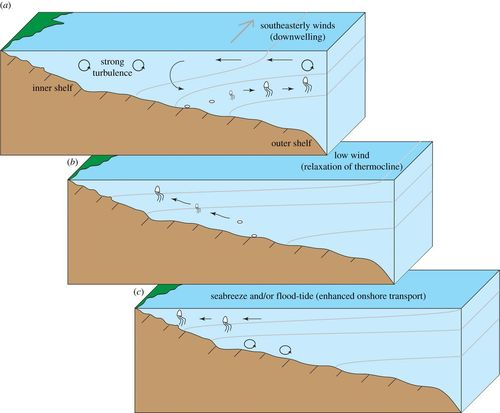
\includegraphics[width=0.6\textwidth]{articuloMedusas2.jpg}
	\caption[Relación entre vientos alisios y medusas]{Relación entre vientos alisios y medusas~\cite{articulomedusas2}.}\label{}
\end{figure}

\section{Proyectos}

Tenemos dos tipos de proyectos principalmente: los que unicamente recogen información de avistamientos y otros que realizan predicciones.

\subsection{Perseus}

Se trata de una web en la que podemos registrar los avistamientos que tengamos introduciendo la localización, el tipo de medusa y la densidad de las misma que hay.
Estos registros se pueden consultar desde la misma página.

Web del proyecto: \href{http://www.perseus-net.eu/en/jellyfish_map/index.html}{http://www.perseus-net.eu/en/jellyfish\_map/index.html}

\subsection{NOAA}

Se trata de una web que ofrece una predicción de la bahía de Chesapeake, cercana a Washington DC. Ofrece a través de un mapa coroplético la probabilidad de la presencia de medusas en cada zona de la bahía.

Web del proyecto: \href{https://ocean.weather.gov/Loops/ocean_guidance.php?model=Sea_Nettles&area=Prob&plot=prob&day=0&loop=1}{NOAA}

\subsection{Infomedusa}

Aplicación para Android y iOS que predice la presencia de medusa en las playas de toda España.

Web del proyecto: \href{https://infomedusa.es/}{https://infomedusa.es/}
\capitulo{7}{Conclusiones y Líneas de trabajo futuras}

Todo proyecto debe incluir las conclusiones que se derivan de su desarrollo. Éstas pueden ser de diferente índole, dependiendo de la tipología del proyecto, pero normalmente van a estar presentes un conjunto de conclusiones relacionadas con los resultados del proyecto y un conjunto de conclusiones técnicas. 
Además, resulta muy útil realizar un informe crítico indicando cómo se puede mejorar el proyecto, o cómo se puede continuar trabajando en la línea del proyecto realizado. 

\section{Lineas futuras}



tratamiento de imagenes


\bibliographystyle{plain}
\bibliography{bibliografia}

\end{document}
